\chapter{Fundamentação Teórica}
Este capítulo busca contextualizar os principais conceitos abordados no presente trabalho, tais como os materiais utilizados como base e também a tecnologia adotada no desenvolvimento do projeto. Ao final, são listados e discutidos alguns trabalhos correlatos.

\section{Estratégia Nacional de Educação Financeira}

A \cite{ENEF} representa uma resposta proativa e estruturada às crescentes demandas de uma sociedade que enfrenta desafios financeiros complexos. Instituída visando aprimorar a conscientização financeira da população brasileira, a ENEF busca não apenas promover a cidadania, mas também equipar os indivíduos com as ferramentas necessárias para tomar decisões financeiras informadas.

Essa estratégia abrange um amplo espectro de áreas de estudo, que vão desde os direitos e deveres básicos até tópicos mais complexos, como investimentos, previdência e planejamento financeiro. A inclusão de temas como poupança, crédito, seguros e consumo demonstra a abordagem abrangente adotada pela \cite{ENEF}. Ao abordar temas tão variados, ela reconhece e enfatiza que a educação financeira é um processo contínuo, que deve começar na infância e continuar ao longo da vida.

A \cite{ENEF} destaca-se por sua abordagem prática, evidenciada por sua ampla variedade de materiais didáticos. Foram elaborados 24 livros especificamente alinhados com sua missão educacional. Cada livro foi cuidadosamente desenvolvido para atender às necessidades de diferentes faixas etárias: 18 destinados ao Ensino Fundamental e os 6 restantes focados no Ensino Médio. Uma característica notável é a separação dos livros em materiais específicos para alunos e guias para professores, garantindo que o conteúdo seja adequadamente direcionado para cada público.

Os primeiros livros pretendem familiarizar os alunos do Ensino Fundamental com conceitos fundamentais de cidadania \cite{ENEF_EF}. Por meio de situações cotidianas, como a organização de uma sala de aula ou a coordenação de eventos escolares, os alunos são introduzidos a princípios de planejamento e organização. Conforme avançam na série, são gradualmente expostos a temas financeiros mais sofisticados, desde o entendimento básico das contas domésticas até a compreensão da origem e da trajetória do dinheiro na sociedade.

Dentre os materiais didáticos, os chamados ``livros-jogo'' se destacam por suas narrativas envolventes. Ao invés de simplesmente transmitir informações, esses livros contam histórias que permitem aos alunos explorar cenários financeiros e entender as consequências de várias decisões. Esse enfoque narrativo é enriquecido por discussões em livros subsequentes, que oferecem \textit{insights} sobre o papel de diferentes instituições financeiras e seu impacto na sociedade.

Nos livros 5~\cite{Livro_ENEF_5_Ano} e 6~\cite{Livro_ENEF_6_Ano} da série ENEF, observa-se uma abordagem pedagógica inovadora e envolvente, que reflete a excelência e o comprometimento em proporcionar uma educação financeira de qualidade. Estes volumes adotam um formato interativo de livro-jogo. Enquanto o jogo digital foca na jogabilidade, o livro-jogo se destaca por sua capacidade de envolver o leitor em uma narrativa rica, permitindo-lhe tomar decisões que influenciam os rumos da história.

A Figura~\ref{fig:figure-1} ilustra um esquema que destaca alguns dos caminhos possíveis que a história pode seguir. Esse diagrama demonstra a complexidade e a diversidade de trajetórias que um jogador pode experimentar, refletindo diferentes escolhas financeiras e suas respectivas consequências.

\begin{figure}[ht]
	\centering
	\caption{Esquema com alguns dos caminhos possíveis da primeiro jogo/história.}
	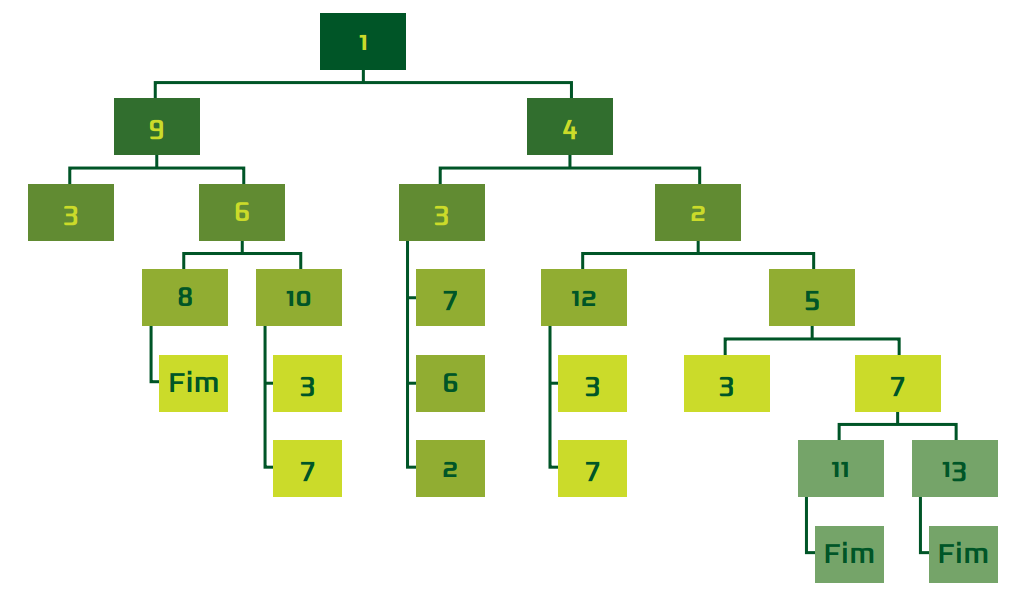
\includegraphics[scale=0.25]{Textuais/Pictures/Picture1.png}
	\fonte{\cite{Livro_ENEF_5_Ano_professor}}\label{fig:figure-1}
\end{figure}

As Figuras~\ref{fig:figure-2} e~\ref{fig:figure-3} retratam momentos cruciais na narrativa do livro-jogo. Em cada figura, o leitor é introduzido a um cenário e, posteriormente, confrontado com duas ou três opções de ação. Cada escolha desencadeia diferentes desenvolvimentos na história, ilustrando as implicações de suas decisões no mundo financeiro.

\begin{figure}[ht]
	\centering
	\caption{Momento de decisão com duas possibilidades de caminhos.}
	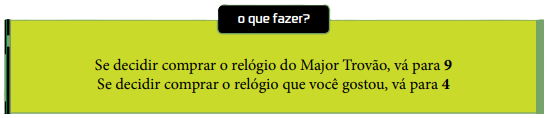
\includegraphics[scale=0.75]{Textuais/Pictures/Picture2.png}
	\fonte{\cite{Livro_ENEF_5_Ano}}\label{fig:figure-2}
\end{figure}

\begin{figure}[ht]
	\centering
	\caption{Momento de decisão com duas possibilidades de caminhos.}
	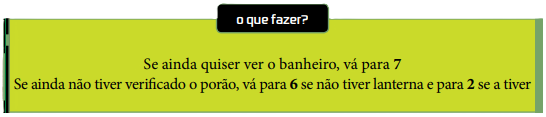
\includegraphics[scale=0.75]{Textuais/Pictures/Picture3.png}
	\fonte{\cite{Livro_ENEF_5_Ano}}\label{fig:figure-3}
\end{figure}

Na continuação da série, principalmente nas fases finais do Ensino Fundamental, a ENEF aprofunda a abordagem, introduzindo conceitos mais avançados e específicos sobre o universo financeiro \cite{ENEF_EM}. Os alunos são expostos a uma variedade de instituições financeiras e suas respectivas funções. Por exemplo, ao aprender sobre bancos, os estudantes ganham experiência sobre operações bancárias, sistemas de crédito e a importância da gestão financeira. Quando o tema é agências de viagens ou hotéis, os alunos são introduzidos ao mundo das transações comerciais, tarifas, reservas e a economia do turismo. Essa abordagem detalhada serve para ampliar o horizonte dos alunos e prepará-los para interações financeiras mais complexas no futuro.

\section{RPG Maker MZ}

O RPG Maker MZ~\cite{RPGMakerMZ} é uma plataforma de desenvolvimento de jogos notavelmente sofisticada, direcionada especificamente para a criação de Role-Playing Games (RPGs). Esta ferramenta, ilustrada na Figura~\ref{fig:rpgmaker-interface}, é equipada com uma interface de usuário intuitiva e um conjunto de recursos predefinidos. Sua concepção tem como objetivo democratizar o processo de desenvolvimento de jogos, fornecendo aos indivíduos, independentemente de seu nível de expertise no design de jogos, os meios necessários para transformar conceitos criativos em realidades interativas.

Inserida neste contexto, a capacidade do RPG Maker MZ de permitir a edição avançada de mapas e a programação de eventos condicionados pela localização geográfica no jogo destaca-se como uma de suas características mais proeminentes. O editor de mapas habilita os usuários a comporem cenários digitais minuciosamente detalhados, que vão desde extensas topografias naturais até ambientes internos complexos. A implementação de eventos baseados em localização é fundamental, atuando como um pilar para a narrativa e as mecânicas lúdicas. Desta maneira, o RPG Maker MZ estabelece um ambiente sinérgico de edição de mapas e administração de eventos, promovendo uma interação harmoniosa entre a estrutura espacial do jogo e sua trama, culminando em uma experiência de jogo coesa, imersiva e cativante~\cite{RPGMakerMZ}.

\begin{figure}[ht]
	\centering
	\caption{Interface do RPG Maker MZ~\cite{RPGMakerMZ}.}
	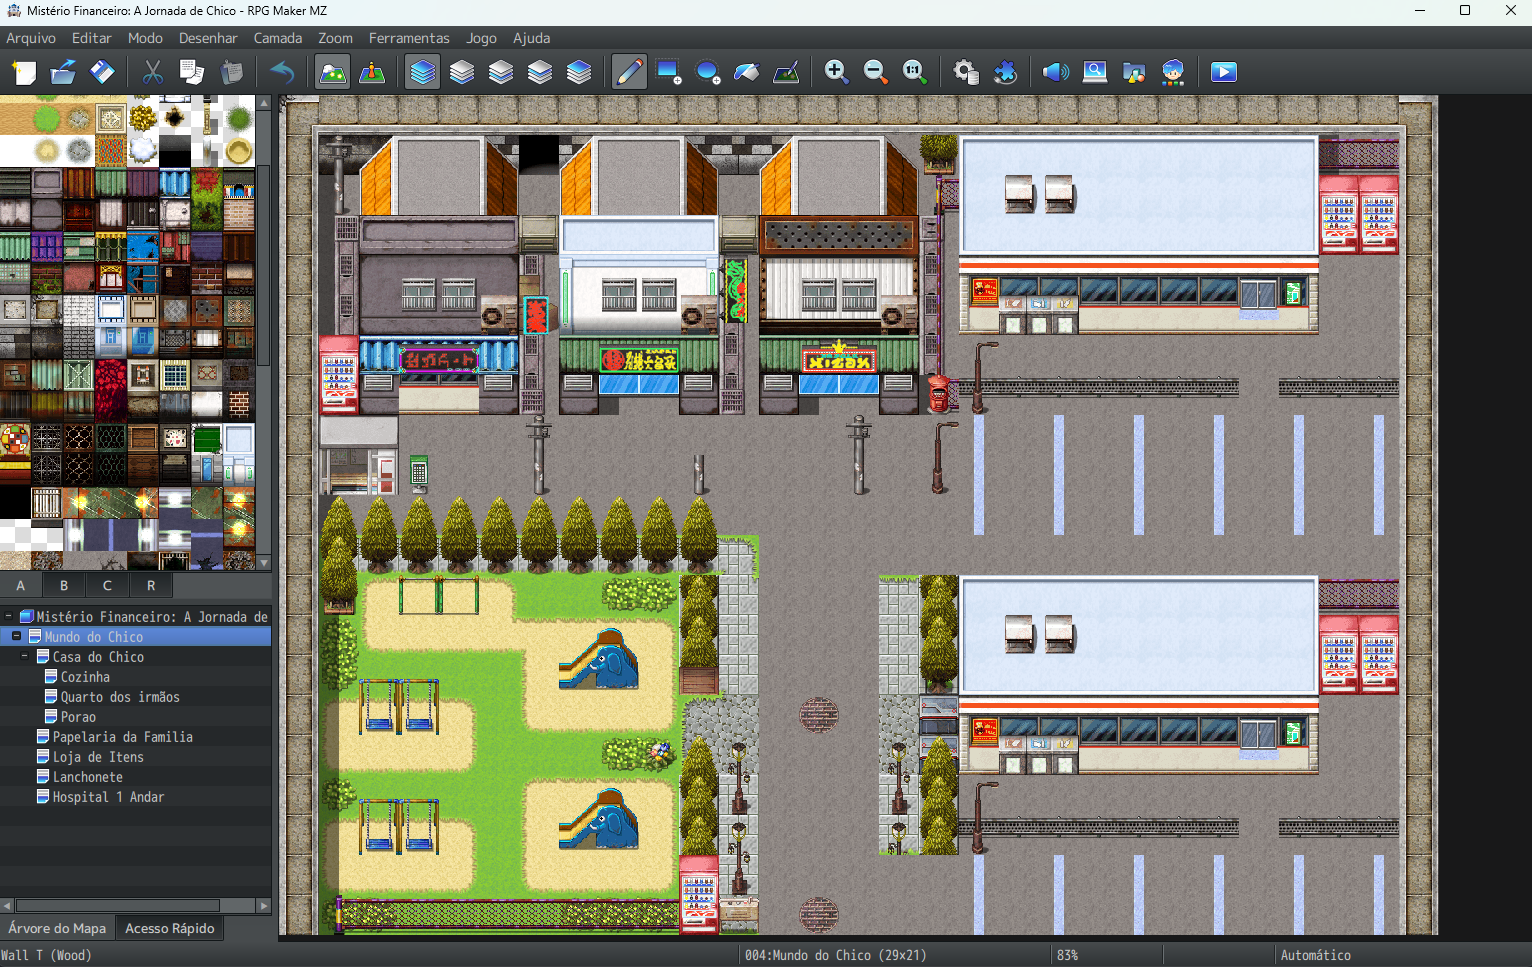
\includegraphics[scale=0.25]{Textuais/Pictures/RPGMaker_Interface.png}
	\fonte{Captura de tela do autor (2023).}\label{fig:rpgmaker-interface}
\end{figure}

\newpage

\subsubsection*{Comandos de evento}
A Figura~\ref{fig:rpgmaker-event-commands} ilustra a interface de usuário do RPG Maker MZ dedicada à configuração dos comandos de evento. Estes comandos são elementos vitais no desenvolvimento de jogos, permitindo a criação de interações narrativas, mecânicas de jogo e controle ambiental. Entre os comandos disponíveis, destacam-se aqueles frequentemente empregados pelos desenvolvedores devido à sua versatilidade e impacto significativo na jogabilidade:

\begin{itemize}
	\item \textit{\textbf{Show Text}}: Exibe texto na tela, com opções de personalização da apresentação;
	\item \textit{\textbf{Show Choices}}: Apresenta escolhas para o jogador, afetando o rumo do jogo;
	\item \textit{\textbf{Control Switches}}: Manipula interruptores que controlam eventos e condições no jogo;
	\item \textit{\textbf{Control Variables}}: Gerencia variáveis para dinâmicas complexas de jogo;
	\item \textit{\textbf{Common Event}}: Controla a chamada de outros eventos, como eventos de cenas do jogo;
	\item \textit{\textbf{Change Gold}}: Altera a quantidade de moeda do jogador, afetando possíveis transações e eventos;
	\item \textit{\textbf{Transfer Player}}: Move o jogador para diferentes localizações dentro do jogo;
	\item \textit{\textbf{Set Movement Route}}: Define rotas específicas para o movimento de personagens ou eventos;
	\item \textit{\textbf{Show Picture}}: Exibe imagens na tela para reforçar narrativas ou ilustrar itens e personagens;
	\item \textit{\textbf{Erase Picture}}: Remove imagens da tela, geralmente utilizada para limpar a interface;
	\item \textit{\textbf{Fadeout Screen}}: Realiza um efeito de transição ao escurecer a tela gradualmente;
	\item \textit{\textbf{Fadein Screen}}: Transição inversa do Fadeout, clareando a tela para o retorno à cena;
	\item \textit{\textbf{Play BGM}}: Inicia a reprodução de música de fundo para ambientação;
	\item \textit{\textbf{Game Over}}: Finaliza o jogo, mostrando a tela de fim de jogo;
	\item \textit{\textbf{Open Menu Screen}}: Abre o menu do jogo para acesso às opções e itens;
	\item \textit{\textbf{Plugin Command}}: Executa comandos de plugins, expandindo as funcionalidades do software.
\end{itemize}

\begin{figure}[ht]
	\centering
	\caption{Comandos de evento disponíveis no RPG Maker MZ~\cite{RPGMakerMZ}.}
	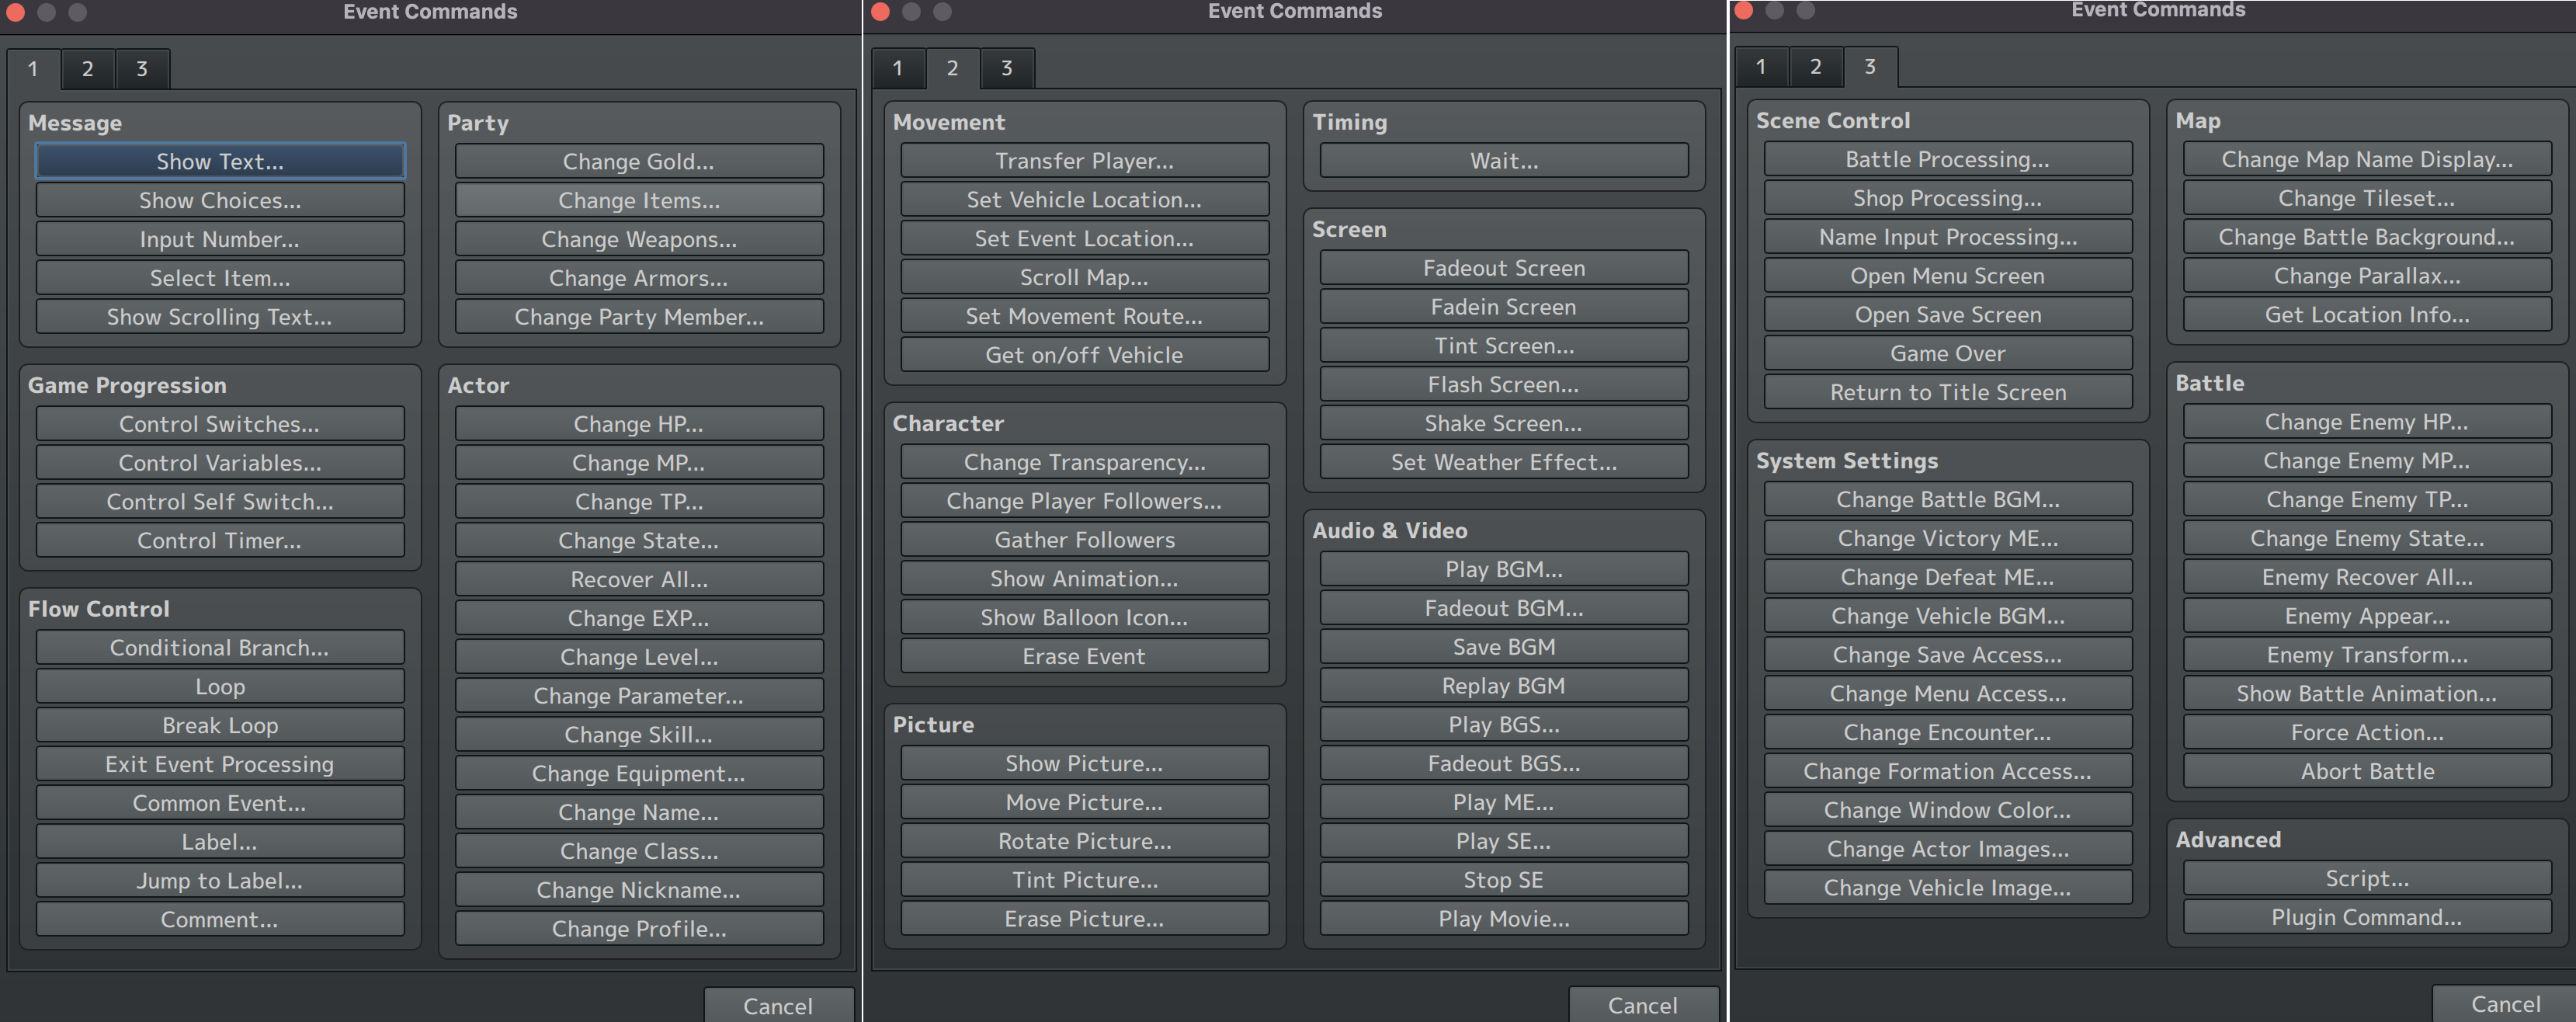
\includegraphics[scale=0.25]{Textuais/Pictures/Event-commands.png}
	\fonte{Captura de tela do autor (2023).}\label{fig:rpgmaker-event-commands}
\end{figure}

\newpage

\subsubsection*{Criador de Personagens}
O RPG Maker MZ~\cite{RPGMakerMZ} contém um módulo dedicado à criação de personagens, demonstrado na Figura~\ref{fig:rpgmaker-criador-personagens}. Esta funcionalidade permite aos usuários compor personagens personalizados através da seleção de atributos distintos como faces, penteados, expressões faciais, vestuário e acessórios. Esta variedade de opções habilita uma personalização detalhada, facilitando a criação de personagens únicos que se alinham com a narrativa e o estilo artístico do jogo.

A interface do criador de personagens, apresentada na Figura~\ref{fig:rpgmaker-criador-personagens}, é projetada para ser intuitiva, guiando os desenvolvedores na configuração dos elementos visuais dos avatares passo a passo. Tal processo não somente estabelece a identidade visual dos personagens, mas também pode influenciar suas interações e papéis dentro da dinâmica do jogo.

\begin{figure}[ht!]
	\centering
	\caption{Interface do criador de personagens no RPG Maker MZ~\cite{RPGMakerMZ}.}
	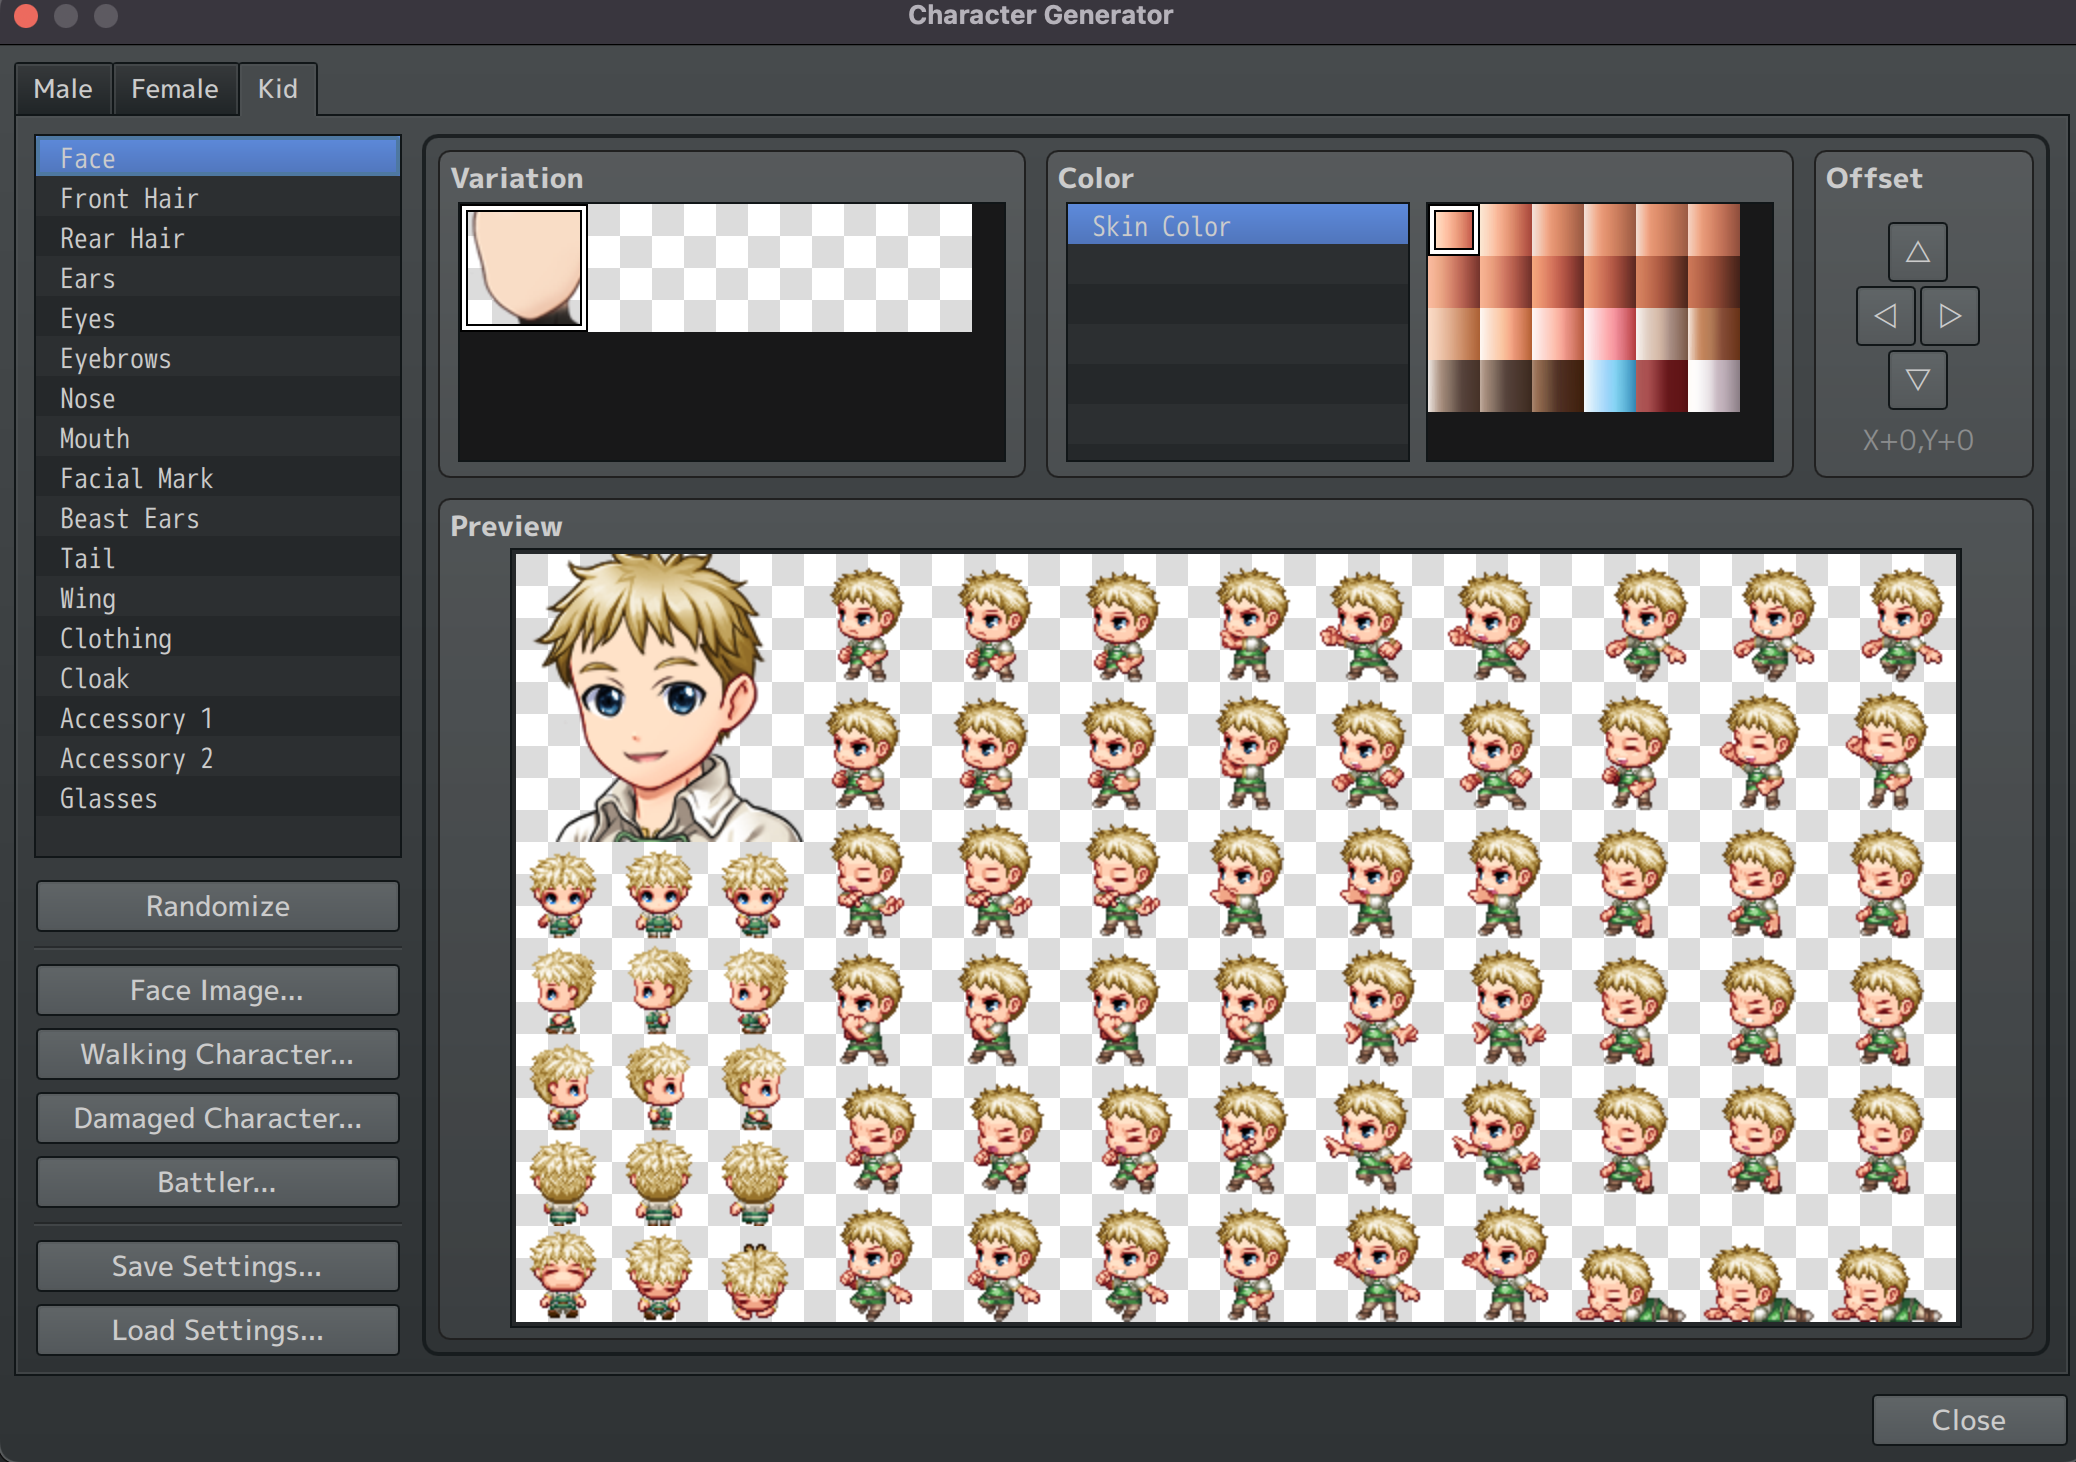
\includegraphics[scale=0.25]{Textuais/Pictures/Picture5.png}
	\fonte{Captura de tela do autor (2023).}\label{fig:rpgmaker-criador-personagens}
\end{figure}

\newpage

\subsubsection*{Banco de Dados}
O banco de dados incorporado ao RPG Maker MZ~\cite{RPGMakerMZ} é um componente central da plataforma, servindo como o núcleo para a gestão de diversos elementos essenciais à criação e ao desenvolvimento do jogo. Como ilustrado na Figura~\ref{fig:rpgmaker-interface-database}, o banco de dados permite o armazenamento e a manipulação de uma vasta gama de dados, incluindo:

\begin{itemize}
	\item \textbf{Actors}: Define os personagens jogáveis, incluindo seus nomes, classes, aparências e equipamentos iniciais;
	\item \textbf{Items}: Permite a criação e configuração de itens que podem ser utilizados pelos personagens, incluindo armas, armaduras, poções e artefatos especiais, cada um com suas propriedades e efeitos definidos;
	\item \textbf{Tilesets}: Conjuntos de tiles que são usados para construir os mapas do mundo do jogo, desde ambientes naturais a construções, proporcionando a base para a criação de cenários diversificados;
	\item \textbf{Common Events}: Eventos que podem ser chamados em diversas circunstâncias dentro do jogo, facilitando a reutilização de lógicas de eventos e a organização do fluxo de jogo;
	\item \textbf{System 1}: Configurações do sistema que incluem a música de fundo e os sons por padrão, as opções de batalha, e outras definições gerais que afetam o comportamento global do jogo;
	\item \textbf{System 2}: Continuação das configurações do sistema onde se podem ajustar os termos utilizados no jogo, os gráficos da janela de comando, entre outras opções que personalizam ainda mais a experiência do jogador.
\end{itemize}

\begin{figure}[ht]
	\centering
	\caption{Interface do Banco de dados do jogo no RPG Maker MZ~\cite{RPGMakerMZ}.}
	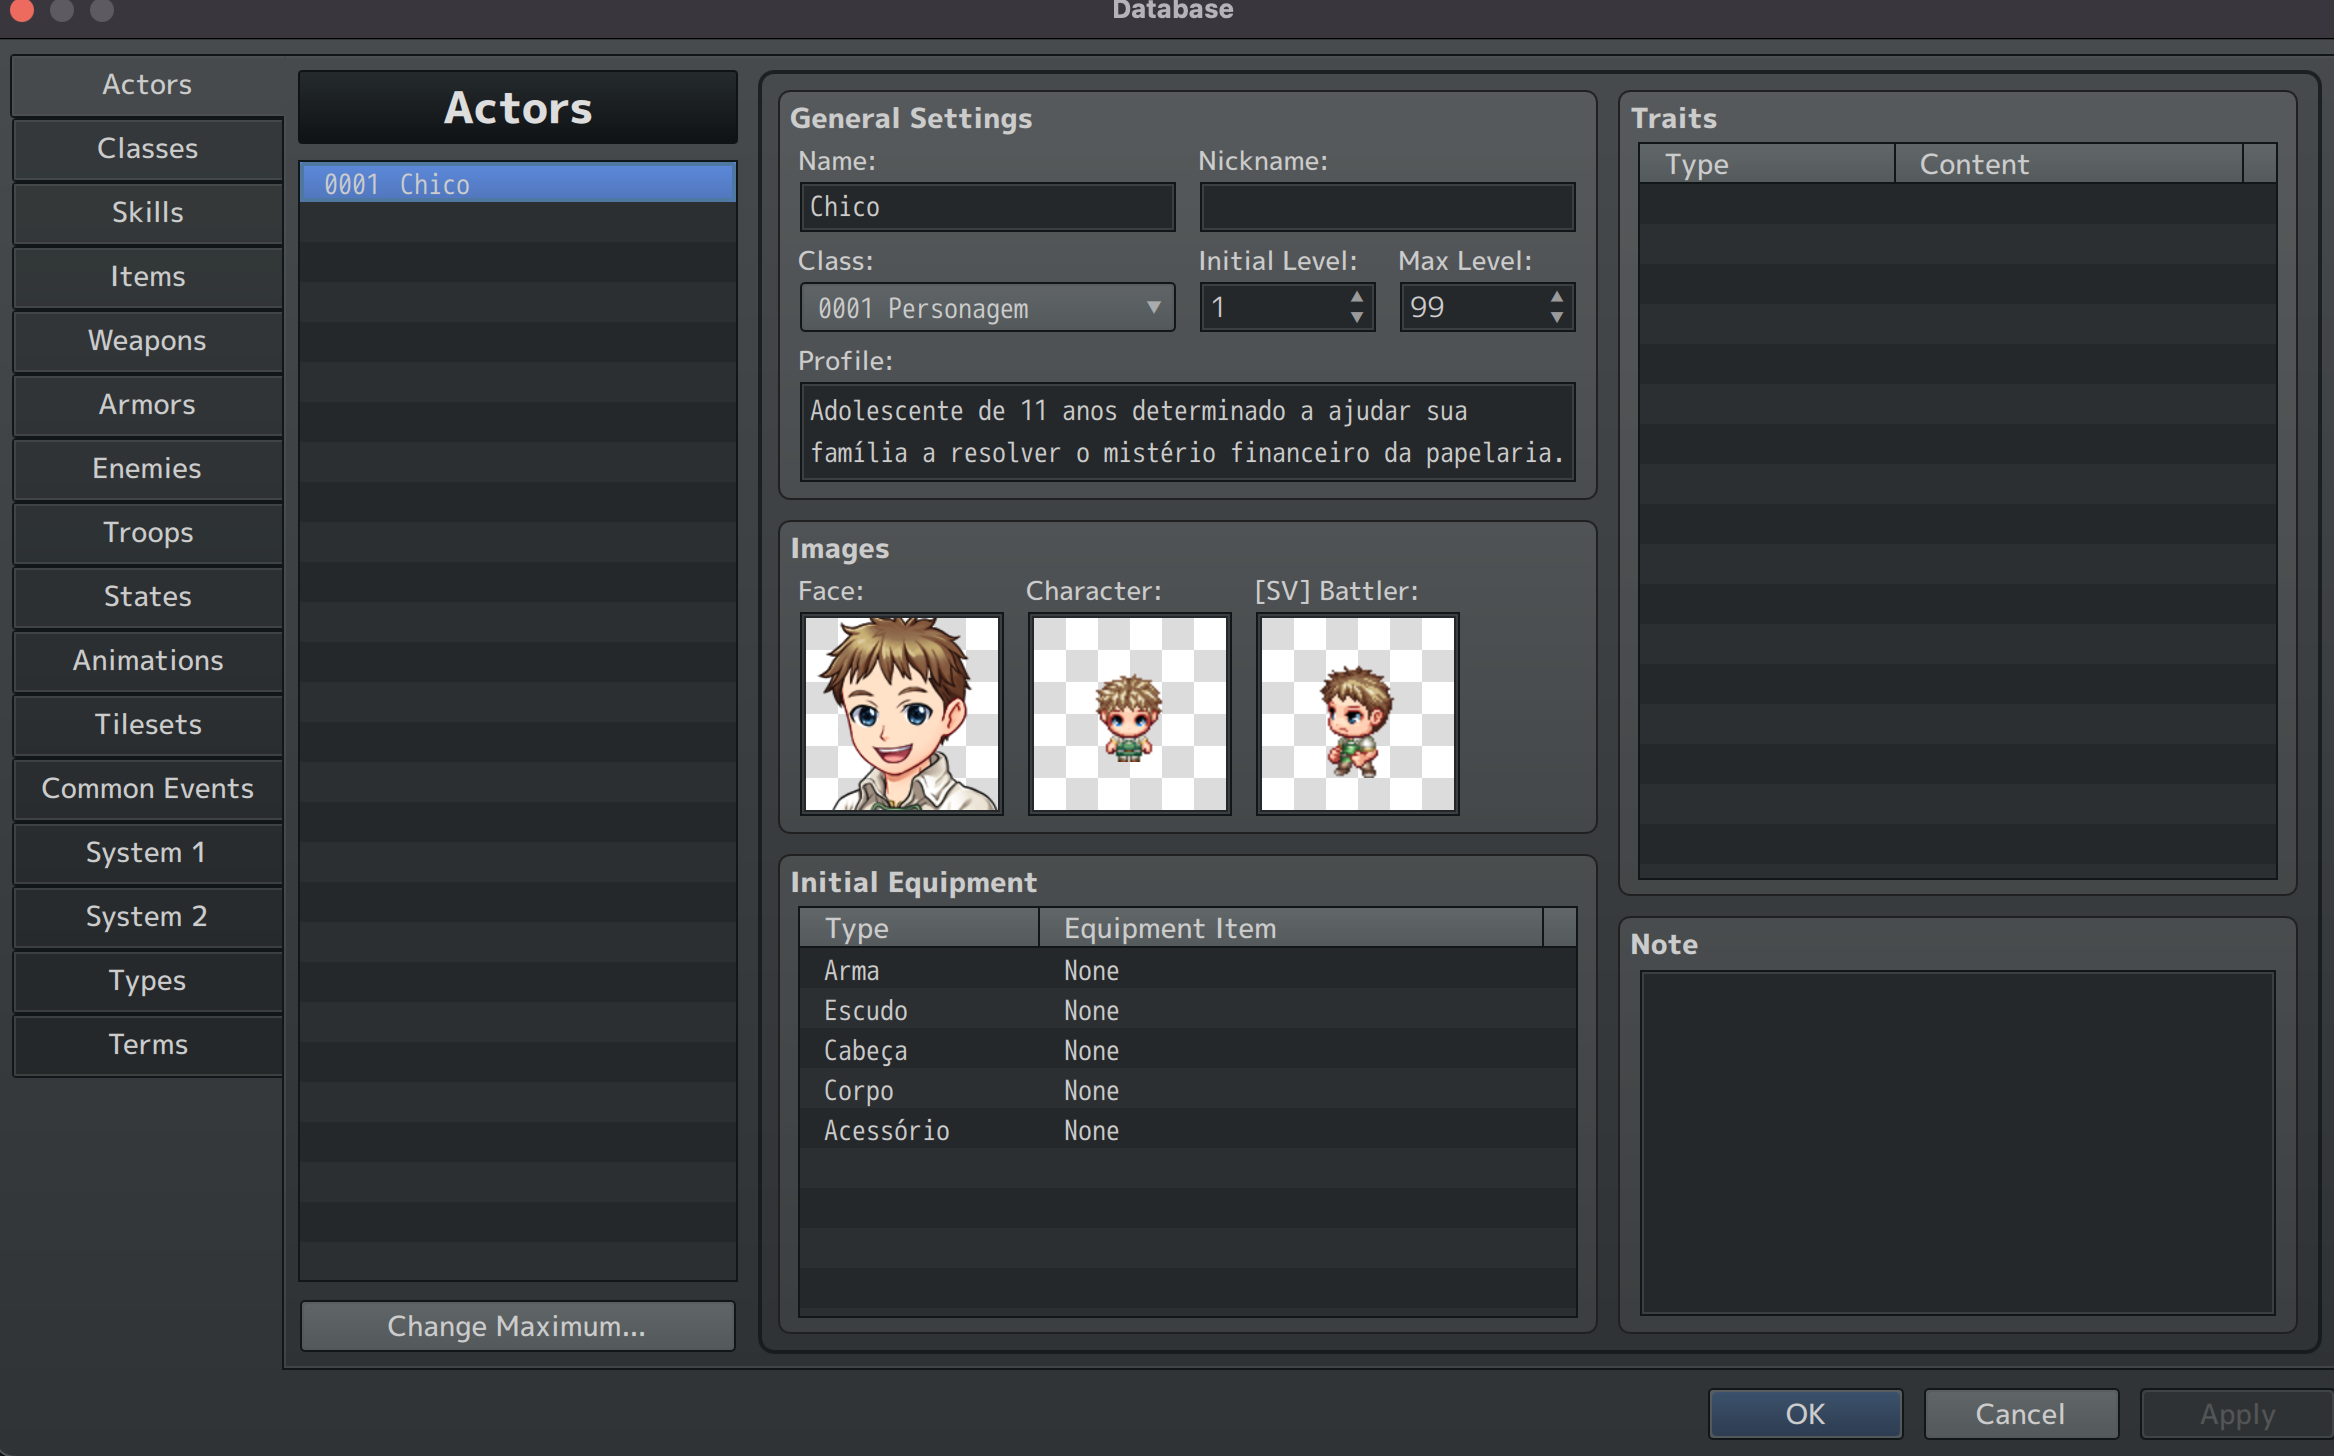
\includegraphics[scale=0.25]{Textuais/Pictures/DataBase.png}
	\fonte{Captura de tela do autor (2023).}\label{fig:rpgmaker-interface-database}
\end{figure}

\newpage

\section{GIMP}

O GIMP (\textit{GNU Image Manipulation Program}) é uma ferramenta de edição de imagens de código aberto, robusta e multiplataforma, que se revela uma escolha eficiente para a edição de \textit{tilesets} utilizados no RPG Maker MZ. Sua funcionalidade de manipulação de imagens permite aos desenvolvedores modificar e criar \textit{tilesets} personalizados, proporcionando um nível adicional de personalização e originalidade aos mapas do jogo. O GIMP suporta uma ampla gama de formatos de arquivo e oferece um leque de ferramentas de edição, desde simples cortes e ajustes de cores até operações complexas de manipulação de camadas e efeitos \cite{GIMP_Documentation}.

\begin{figure}[ht]
	\centering
	\caption{Interface de edição de imagem do \cite{GIMP_Documentation}.}
	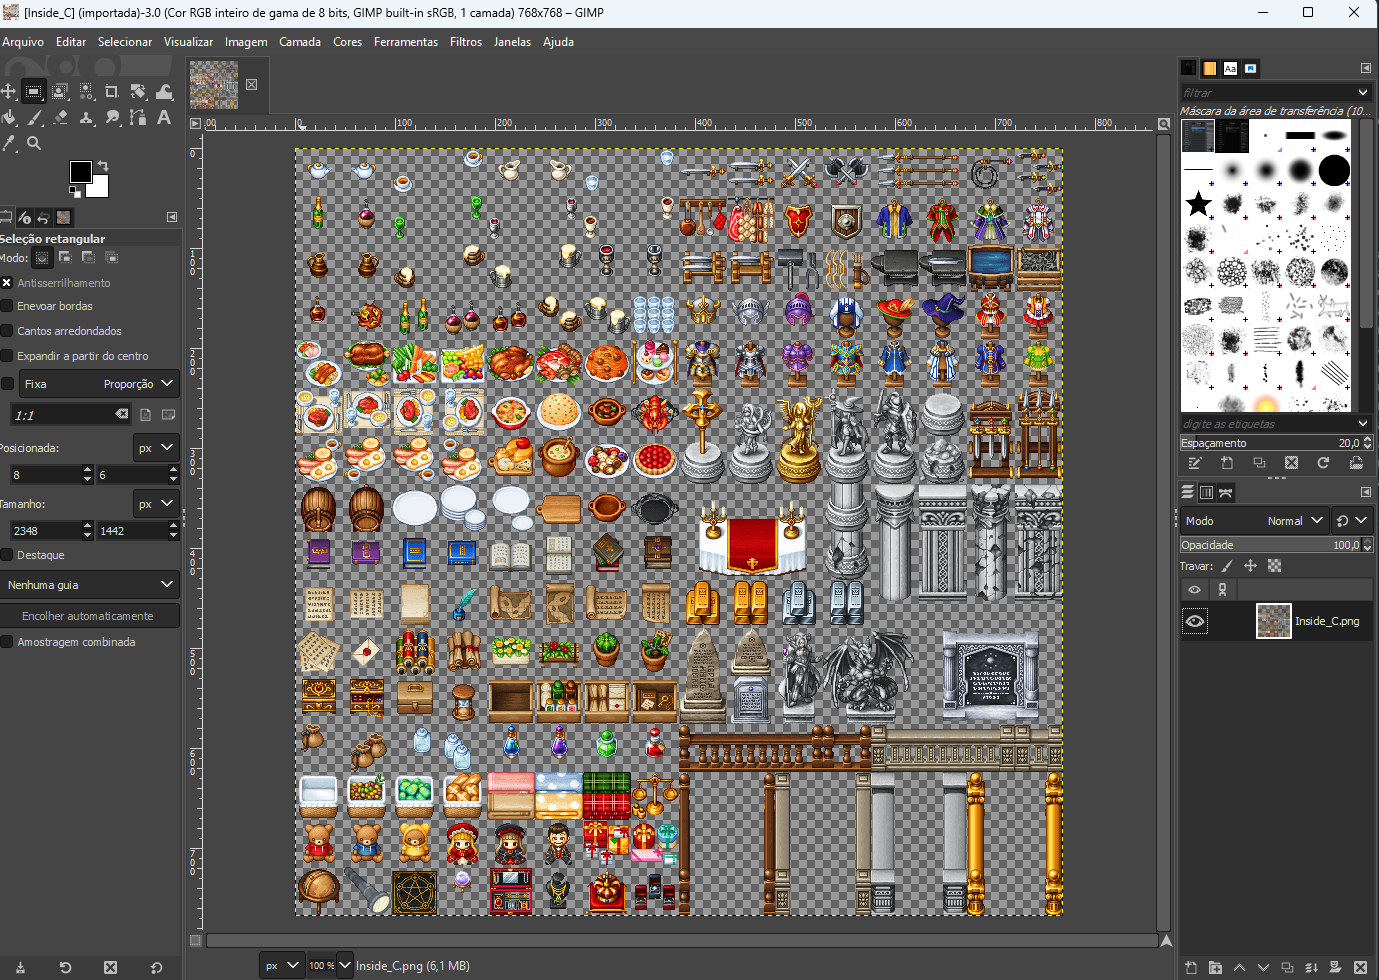
\includegraphics[scale=0.3]{Textuais/Pictures/Gimp.png}
	\fonte{Captura de tela do autor (2023).}\label{fig:gimp-interface}
\end{figure}

\section{Trabalhos Correlatos}
Esta seção apresenta alguns trabalhos que, de alguma forma, se correlacionam com o presente estudo, oferecendo uma perspectiva sobre as diversas abordagens em jogos educativos focados na educação financeira.

\subsection{Debt Maze}
\label{subsec:debt-maze}

O \textit{Debt Maze}~\cite{Debt_Maze} representa um marco na integração de conceitos financeiros em jogos digitais, introduzindo uma experiência interativa que se adapta aos diferentes níveis de conhecimento financeiro dos usuários. O jogo desafia os jogadores com um labirinto que simboliza o percurso das decisões financeiras, utilizando conceitos como empréstimos, juros e pagamentos em atraso para promover a alfabetização financeira. Como ilustrado na Figura~\ref{fig:debt-maze-1}, o jogo encoraja o jogador a melhorar sua pontuação de crédito para receber recompensas e habilidades que facilitam a navegação no labirinto, refletindo a importância de um bom histórico financeiro.

Além disso, como mostrado na Figura~\ref{fig:debt-maze-2}, o jogo apresenta dinâmicas que envolvem caixas eletrônicos, onde os jogadores podem realizar saques de diferentes quantidades de dinheiro. Rotas otimizadas no jogo recompensam o jogador com acessos a caixas eletrônicos benéficos, simbolizando a vantagem do conhecimento financeiro e as recompensas por tomar decisões corretas.

Diferentemente, o jogo desenvolvido neste trabalho destaca-se por seu foco no público brasileiro, alinhando-se às diretrizes da Estratégia Nacional de Educação Financeira (ENEF) e empregando o português como idioma principal. A relevância de um jogo em português é evidente, uma vez que a barreira linguística pode comprometer a aplicabilidade de um jogo em inglês no contexto educacional brasileiro. Em contraste com o labirinto metafórico do \textit{Debt Maze}, o jogo proposto neste estudo baseia-se em cenários realistas e utiliza ferramentas interativas para simular decisões financeiras, tornando o aprendizado mais próximo à realidade vivenciada pelas crianças no Brasil. Isso evidencia a importância de desenvolver uma educação financeira que esteja em sintonia com o contexto sociocultural dos estudantes do Ensino Fundamental.

\begin{figure}[ht]
	\centering
	\caption{Interface do \textit{Debt Maze} demonstrando recompensas por alta pontuação de crédito.}
	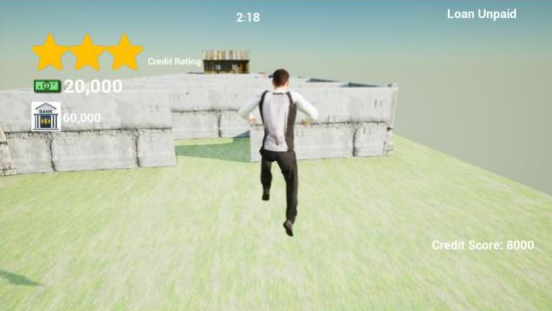
\includegraphics[scale=0.9]{Textuais/Pictures/debt-maze-1.png}
	\fonte{\textit{Debt Maze}~\cite{Debt_Maze}.}\label{fig:debt-maze-1}
\end{figure}

\begin{figure}[ht]
	\centering
	\caption{Interface do \textit{Debt Maze} com a mecânica de saques em caixas eletrônicos.}
	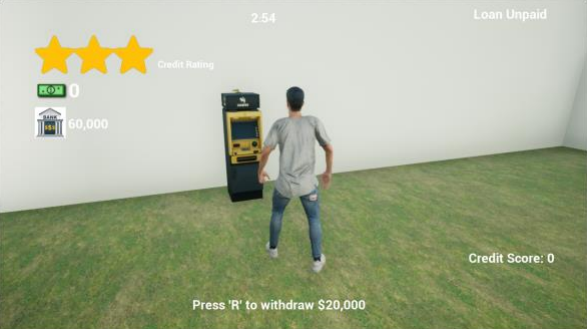
\includegraphics[scale=0.8]{Textuais/Pictures/debt-maze-2.png}
	\fonte{\textit{Debt Maze}~\cite{Debt_Maze}.}\label{fig:debt-maze-2}
\end{figure}

\newpage

\subsection{PlanCash}
\label{subsec:plancash}

O \textit{PlanCash}~\cite{mariano2020educaccao} é um jogo de tabuleiro educativo que busca ensinar conceitos de matemática e gestão financeira para crianças. Como mostrado na Figura~\ref{fig:plancash-1}, o manual do jogo explica as regras e os objetivos, orientando os jogadores a cumprir tarefas após cada movimento e a avançar no tabuleiro baseando-se em indicadores financeiros. A estrutura do jogo é projetada para engajar os jovens jogadores em atividades que refletem situações econômicas do mundo real, promovendo o aprendizado por meio da interação lúdica.

A Figura~\ref{fig:plancash-2} ilustra o tabuleiro do \textit{PlanCash}, onde os jogadores avançam por um caminho repleto de diferentes desafios econômicos. As células do tabuleiro representam diversas situações financeiras, como ganhos, despesas, e oportunidades de investimento, incentivando as crianças a tomarem decisões informadas e a desenvolverem habilidades de planejamento financeiro.

Contrastando com \textit{PlanCash}, o jogo desenvolvido neste trabalho avança na direção de uma proposta digital no estilo RPG, que tende a ser mais atraente para a geração atual de crianças acostumadas ao uso de tecnologias interativas. Diferente de um tabuleiro físico, a abordagem digital propicia um ambiente dinâmico e imersivo. Isso permite que os jogadores explorem mundos virtuais e enfrentem desafios financeiros de uma forma mais envolvente e interativa, alinhando o aprendizado financeiro com as tendências tecnológicas contemporâneas e as preferências do público infantojuvenil.

\begin{figure}[ht]
	\centering
	\caption{Manual do \textit{PlanCash}, destacando as instruções e regras do jogo.}
	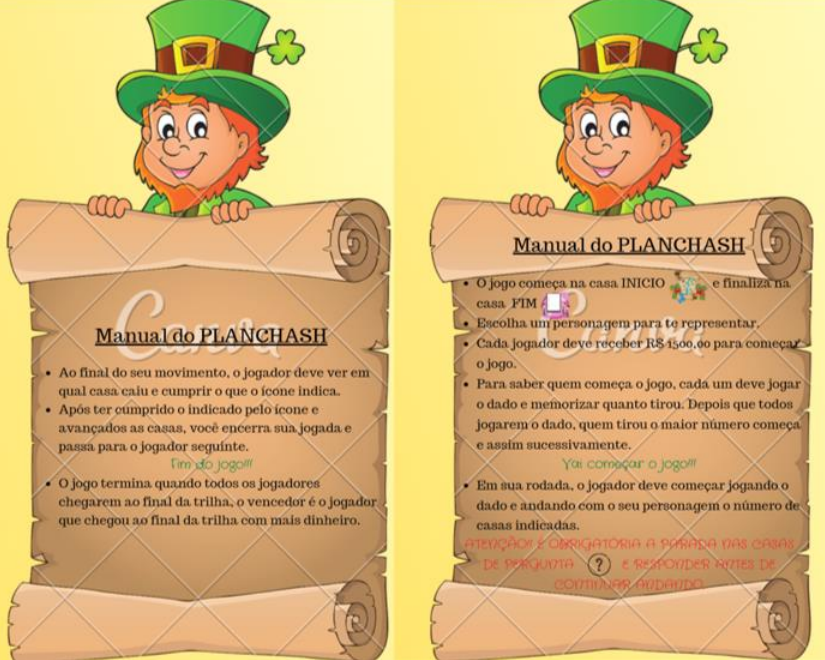
\includegraphics[scale=0.45]{Textuais/Pictures/Plancash-1.png}
	\fonte{\textit{PlanCash}~\cite{mariano2020educaccao}.}\label{fig:plancash-1}
\end{figure}

\begin{figure}[ht]
	\centering
	\caption{Tabuleiro do \textit{PlanCash}, exibindo o percurso e as diferentes células financeiras que os jogadores encontram.}
	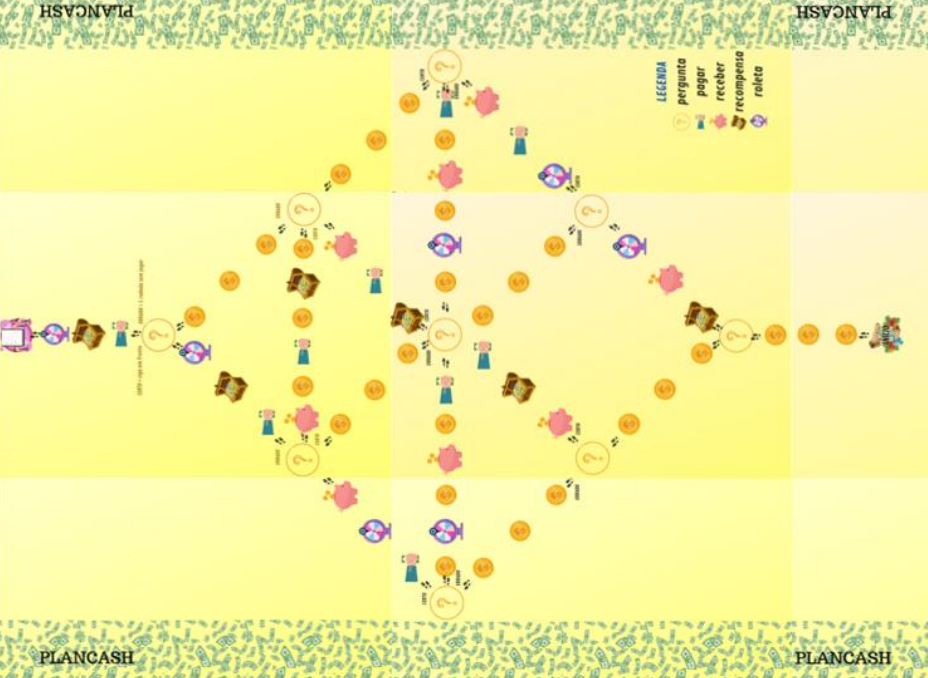
\includegraphics[scale=0.45]{Textuais/Pictures/Plancash-2.png}
	\fonte{\textit{PlanCash}~\cite{mariano2020educaccao}.}\label{fig:plancash-2}
\end{figure}

\newpage

\subsection{Finance Game}
\label{subsec:finance-game}

O \textit{Finance Game} \cite{Finance_Game}, representado na Figura~\ref{fig:finance-game-1}, é um ambiente simulado que desafia as crianças a tomar decisões financeiras equilibradas em um cenário que espelha a vida adulta. O jogo se desenrola em uma cidade virtual, onde o jogador deve administrar suas finanças pessoais e profissionais, lidando com o equilíbrio entre trabalho, lazer, educação e saúde, conforme ilustrado na Figura~\ref{fig:finance-game-2}. As escolhas feitas no jogo afetam diretamente um parâmetro chamado "Qualidade de Vida", que reflete o sucesso das decisões financeiras do jogador, variando entre zero e cem.

Em contrapartida, o jogo desenvolvido neste trabalho, embora também voltado para a educação financeira, direciona-se especificamente ao entendimento e experiência das crianças. Enquanto o \textit{Finance Game} foca em simular a vida adulta para promover o aprendizado financeiro, o projeto atual busca envolver os jogadores em cenários lúdicos que são mais próximos do seu universo infantil. A abordagem do novo jogo é desenhada para facilitar a compreensão dos conceitos financeiros, adaptando-se ao nível cognitivo e à vivência do público infantil, tornando o aprendizado não apenas prático mas também significativo para suas experiências diárias.

\begin{figure}[ht]
	\centering
	\caption{Tela de seleção de avatar e introdução ao \textit{Finance Game}, destacando a interatividade e as escolhas iniciais que o jogador deve fazer.}
	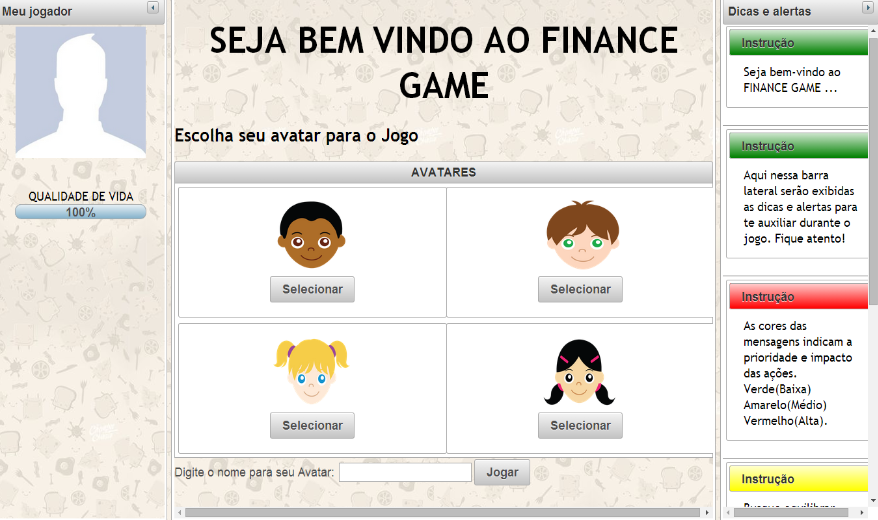
\includegraphics[scale=0.46]{Textuais/Pictures/Finance-game-1.png}
	\fonte{\textit{Finance Game} \cite{Finance_Game}.}\label{fig:finance-game-1}
\end{figure}

\begin{figure}[ht]
	\centering
	\caption{Cenário do mercado no \textit{Finance Game}, onde o jogador enfrenta decisões sobre compras e gestão de recursos, promovendo habilidades de planejamento e raciocínio matemático.}
	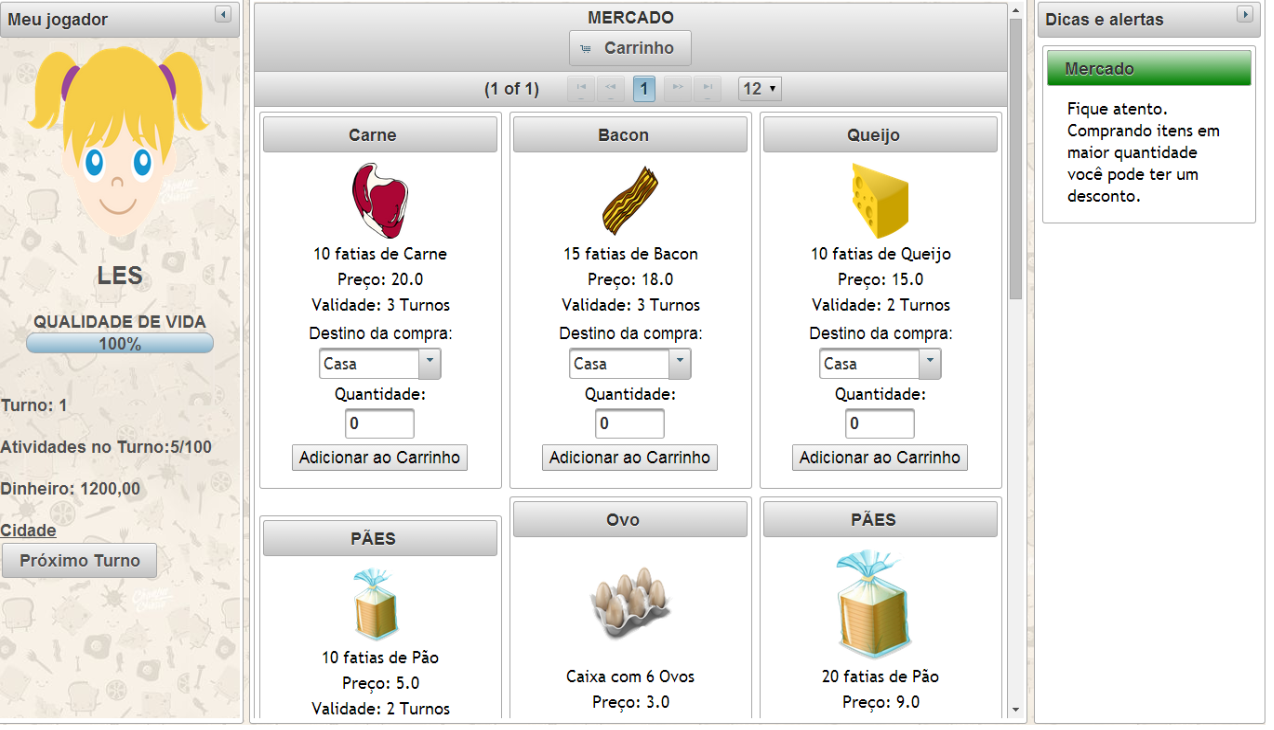
\includegraphics[scale=0.3]{Textuais/Pictures/Finance-game-2.png}
	\fonte{\textit{Finance Game} \cite{Finance_Game}.}\label{fig:finance-game-2}
\end{figure}

\newpage

\subsection{InvestPlay}
\label{subsec:investplay}

O \textit{InvestPlay} \cite{santos2020investplay}, é um jogo educativo digital que simula um ambiente financeiro interativo, ensinando crianças e adolescentes a gerenciar ativos e passivos de forma lúdica. As instruções iniciais (Figura~\ref{fig:invest-play-1}) estabelecem as regras do jogo e introduzem os jogadores à mecânica de avanço no tabuleiro, que é alcançado ao responder perguntas relacionadas à educação financeira, investimentos e empreendedorismo.

A Figura~\ref{fig:invest-play-2} apresenta uma cena do jogo, onde o jogador navega pelo tabuleiro 3D, encarando os desafios financeiros representados em cada casa. A imersão do jogador é reforçada pela visualização do personagem no ambiente do jogo e pela interação direta com elementos que simbolizam decisões financeiras reais.

Em comparação, o projeto atual expande o conceito ao propor um RPG educacional, que é mais atrativo para o público infantil devido à sua natureza narrativa e interativa. Enquanto o \textit{InvestPlay} foca em perguntas e respostas para ensinar conceitos financeiros, o RPG imerge as crianças em histórias que contextualizam cada decisão econômica dentro de um enredo envolvente, reforçando o aprendizado através da experiência direta e da consequência das ações no mundo do jogo.

\begin{figure}[ht]
	\centering
	\caption{Tela de instruções do \textit{InvestPlay}, onde são apresentadas as regras do jogo e a dinâmica de progressão pelo tabuleiro.}
	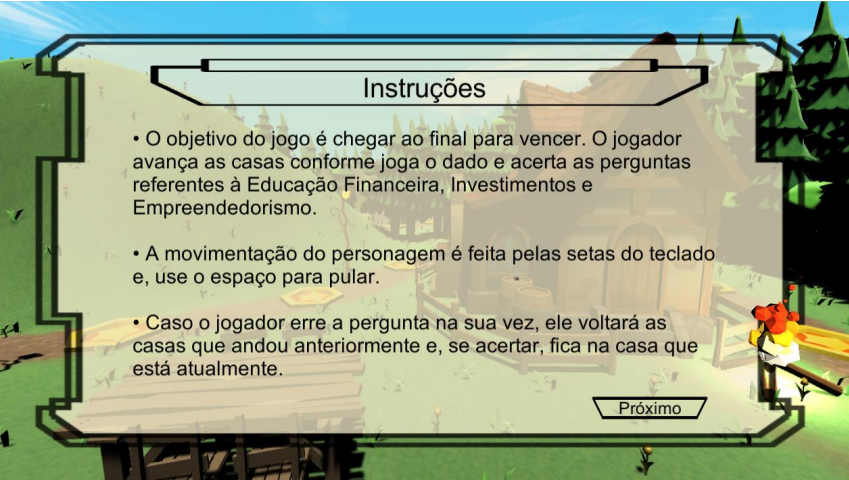
\includegraphics[scale=0.6]{Textuais/Pictures/invest-play-1.png}
	\fonte{\textit{InvestPlay} \cite{santos2020investplay}.}\label{fig:invest-play-1}
\end{figure}

\begin{figure}[ht]
	\centering
	\caption{Jogabilidade do \textit{InvestPlay} mostrando o personagem no tabuleiro e a representação visual das casas que simbolizam diferentes desafios financeiros.}
	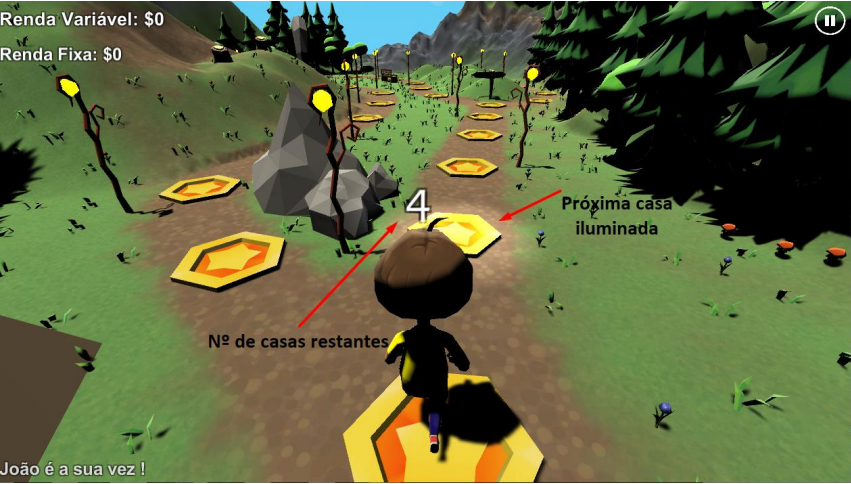
\includegraphics[scale=0.6]{Textuais/Pictures/invest-play-2.png}
	\fonte{\textit{InvestPlay} \cite{santos2020investplay}.}\label{fig:invest-play-2}
\end{figure}

\newpage

\subsection{Considerações sobre os Trabalhos Correlatos}

A análise dos trabalhos correlatos desvenda um diversificado panorama de estratégias lúdicas aplicadas à educação financeira. Cada jogo educativo examinado oferece uma abordagem única para o ensino de conceitos financeiros, refletindo a versatilidade da gamificação como ferramenta pedagógica. A comparação desses jogos, detalhada na Tabela~\ref{tab:comparativo-trabalhos}, evidencia as escolhas metodológicas e pedagógicas distintas que cada um adota, enfatizando a importância de adaptar tanto o conteúdo quanto a abordagem ao público-alvo.

O \textit{Debt Maze}~\ref{subsec:debt-maze}, por exemplo, utiliza a metáfora de um labirinto para simbolizar o percurso das decisões financeiras, adequado para um público mais amplo. O \textit{PlanCash}~\ref{subsec:plancash}, em contraste, emprega o formato tradicional de jogo de tabuleiro, focando no público infantil e integrando elementos educacionais clássicos com a gamificação. O \textit{Finance Game}~\ref{subsec:finance-game} avança na simulação da vida adulta, enquanto o \textit{InvestPlay}~\ref{subsec:investplay} concentra-se em um ambiente interativo de perguntas e respostas.

O jogo desenvolvido neste trabalho busca transcender essas abordagens, almejando uma imersão mais profunda e uma conexão direta com a realidade do público infantil brasileiro. Ao contrário dos jogos mencionados, que não são especificamente alinhados com a Estratégia Nacional de Educação Financeira (ENEF), o novo jogo propõe uma experiência alinhada com os princípios da ENEF e com a linguagem e a cultura brasileira, utilizando o formato de RPG para engajar as crianças de forma mais atraente e interativa. As Figuras~\ref{fig:debt-maze-1}, \ref{fig:debt-maze-2}, \ref{fig:plancash-1}, \ref{fig:plancash-2}, \ref{fig:finance-game-1}, e \ref{fig:finance-game-2} fornecem uma visão visual das diferentes interfaces e estilos de jogo que esses jogos empregam.

Este enfoque no RPG é concebido para tornar o aprendizado financeiro não apenas acessível e pertinente, mas também uma parte integrante da narrativa e do crescimento do personagem dentro do jogo, visando uma internalização mais eficaz e duradoura dos conceitos financeiros.

\begin{table}[!htbp]
	\centering
	\renewcommand{\arraystretch}{1.3}
	\caption{Comparativo Aprofundado dos Trabalhos Correlatos}%
	\label{tab:comparativo-trabalhos}
	\begin{tabular}{| L{3cm} | L{2.7cm} | L{2.7cm} | L{2.7cm} | L{2.7cm} |}
		\hline
		\textbf{Aspecto}                   & \textbf{Debt Maze} & \textbf{PlanCash}                  & \textbf{Finance Game} & \textbf{InvestPlay}    \\
		\hline
		\hline
		\textbf{Público-Alvo}              & Adulto             & Infantil                           & Adulto                & Infantil a Adolescente \\
		\hline
		\textbf{Metodologia}               & Labirinto          & Jogo de Tabuleiro                  & Simulação             & Perguntas e Respostas  \\
		\hline
		\textbf{Abordagem Pedagógica}      & Gamificação        & Gamificação e Educação Tradicional & Simulação Realista    & Dinâmica Interativa    \\
		\hline
		\textbf{Idioma}                    & Inglês             & Português                          & Português             & Português              \\
		\hline
		\textbf{Realismo vs. Metáfora}     & Metáfora           & Realismo                           & Realismo              & Realismo               \\
		\hline
		\textbf{Contextualização Cultural} & Não                & Não                                & Não                   & Sim                    \\
		\hline
		\textbf{Imersão Narrativa}         & Baixa              & Baixa                              & Média                 & Alta                   \\
		\hline
		\textbf{Baseado na ENEF}           & Não                & Não                                & Não                   & Não                    \\
		\hline
	\end{tabular}
	\vspace{2mm}
	\fonte{Elaborado pelo autor (2023).}
\end{table}